%% abtex2-modelo-slides.tex, v-1.0 gfabinhomat
%% Copyright 2012-2013 by abnTeX2 group at http://abntex2.googlecode.com/ 
%%
%% This work may be distributed and/or modified under the
%% conditions of the LaTeX Project Public License, either version 1.3
%% of this license or (at your option) any later version.
%% The latest version of this license is in
%%   http://www.latex-project.org/lppl.txt
%% and version 1.3 or later is part of all distributions of LaTeX
%% version 2005/12/01 or later.
%%
%% This work has the LPPL maintenance status `maintained'.
%% 
%% The Current Maintainer of this work is Fábio Rodrigues Silva, 
%% member of abnTeX2 team, led by Lauro César Araujo. 
%% Further information are available on 
%% http://abntex2.googlecode.com/
%%
%% This work consists of the files abntex2-modelo-slides.tex, 
%% abntex2-modelo-references.bib and abntex2-modelo-marca.pdf
%%
%% Modelo desenvolvido por Fábio Rodrigues Silva (gfabinhomat@gmail.com)
%% Mais informações podem ser obtidas no guia do usuário Beamer 
%% (http://linorg.usp.br/CTAN/macros/latex/contrib/beamer/doc/beameruserguide.pdf)
%% Informações rápidas podem ser acessadas em http://en.wikibooks.org/wiki/LaTeX/Presentations


% Apresentações em widescreen. Outros valores possíveis: 1610, 149, 54, 43 e 32.
% Por padrão, as apresentações são no formato 4:3 (sem o aspectratio).
\documentclass[aspectratio=169]{beamer}	 	

\usetheme{Pittsburgh}
\usecolortheme{default}
\usefonttheme[onlymath]{serif}			% para fontes matemáticas
% Enconte mais temas e cores em http://www.hartwork.org/beamer-theme-matrix/ 
% Veja também http://deic.uab.es/~iblanes/beamer_gallery/index.html

% Customizações de Cores: fg significa cor do texto e bg é cor do fundo
\setbeamercolor{normal text}{fg=black}
\setbeamercolor{alerted text}{fg=red}
\setbeamercolor{author}{fg=blue}
\setbeamercolor{institute}{fg=blue}
\setbeamercolor{date}{fg=green}
\setbeamercolor{frametitle}{fg=red}
\setbeamercolor{framesubtitle}{fg=brown}
\setbeamercolor{block title}{bg=blue, fg=white}		%Cor do título
\setbeamercolor{block body}{bg=gray, fg=darkgray}	%Cor do texto (bg= fundo; fg=texto)

% ---
% PACOTES
% ---
\usepackage[alf]{abntex2cite}		% Citações padrão ABNT
\usepackage[brazil]{babel}		% Idioma do documento
\usepackage{cmap}			% Mapear caracteres especiais no PDF
\usepackage{color}			% Controle das cores
\usepackage[T1]{fontenc}		% Selecao de codigos de fonte.
\usepackage{graphicx}			% Inclusão de gráficos
\usepackage[utf8]{inputenc}		% Codificacao do documento (conversão automática dos acentos)

\usepackage{txfonts}			% Fontes virtuais
\usepackage{epstopdf}
% ---

% --- Informações do documento ---
\title{\emph{Cymbopognon nardus (L.) Rendle} - Citronela}
\author{Chrystian de Sousa Guth}
\institute{Universidade Federal de Santa Catarina
		\par
		Centro Tecnológico - CTC
	    \par
	    Departamento de Informática e Estatística
	    \par
	    Curso de Bacharelado em Ciências da Computação}
\date{\today}
% ---

% ----------------- INÍCIO DO DOCUMENTO --------------------------------------
\begin{document}

% ----------------- NOVO SLIDE --------------------------------
\begin{frame}

\begin{minipage}{1\linewidth}
  \centering
  \begin{tabular}{cc}
    \begin{tabular}{c}
      \includegraphics[width=3.0cm]{horizontal_fundo_claro.eps}
    \end{tabular}
    &
    \begin{tabular}{c}
      \textbf{Centro de Ciências da Saúde} \\ \textbf{Departamento de Enfermagem}
      \\\textbf{Plantas Medicinais nas Práticas de Saúde}
    \end{tabular}
  \end{tabular}
\end{minipage}

\titlepage

\end{frame}

% ----------------- NOVO SLIDE --------------------------------
\begin{frame}{Sumário}
\tableofcontents
\end{frame}

% ----------------- NOVO SLIDE --------------------------------
\section{Introdução}

\begin{frame}{Introdução}

\begin{itemize}
	\item Plantas Medicinais \pause
	\item Manutenção da Vida \pause
	\item Nutrição \pause
	\item Tratamento de Enfermidades
\end{itemize}

\end{frame}

% ----------------- NOVO SLIDE --------------------------------
\section{Cymbopognon nardus}
\begin{frame}
\frametitle{A Planta}
\framesubtitle{\emph{Cymbopognon nardus}}

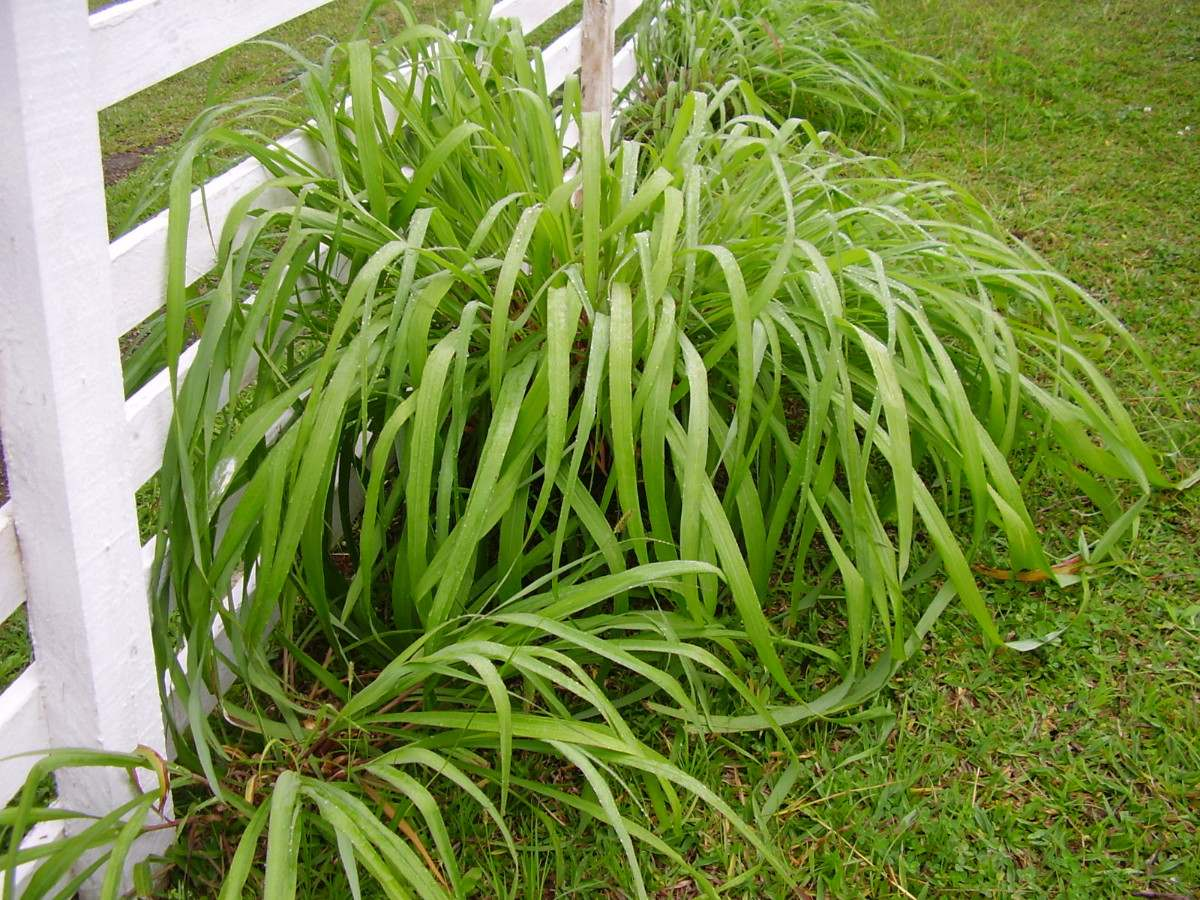
\includegraphics[scale=0.2]{imgs/citronela.jpg} 

\end{frame}

% ----------------- NOVO SLIDE --------------------------------
\begin{frame}
\frametitle{Citronela}
\framesubtitle{Classificação Científica}
	
	\begin{itemize}

		\item \textbf{Reino:}	\emph{Plantae} \pause
	
		\item \textbf{Divisão:} \emph{Magnoliophyta} \pause
	
		\item \textbf{Classe:}	\emph{Liliopsida} \pause
	
		\item \textbf{Ordem:}	\emph{Poales} \pause
	
		\item \textbf{Família:}	 \emph{Poaceae} \pause
	
		\item \textbf{Gênero:}	\emph{Cymbopogon Spreng.} \pause
	
		\item \textbf{Espécie:}	 \emph{C. nardus.}

	\end{itemize}

\end{frame}


% ----------------- NOVO SLIDE --------------------------------
\begin{frame}
\frametitle{Citronela}
\framesubtitle{Sinônimos e Região de Origem}
	\begin{minipage}{0.49\textwidth}
		\begin{itemize}
			\item	\emph{Cymbopognon nardus} \pause
			\item \emph{Cymbopognon afronardus} \pause
			\item Citronela Falsa \pause
			
			\begin{itemize}
				\item \emph{Citronella mucronata} 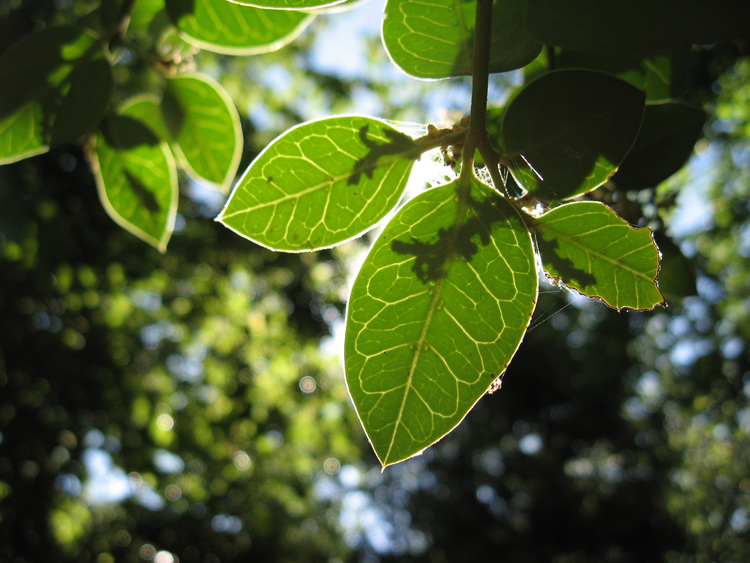
\includegraphics[scale=0.4]{imgs/mucronata.jpg} \pause
			\end{itemize}		
			
			\item Capim Citronela \pause
			
			\item  \textbf{Origem: } Ásia Tropical
		\end{itemize}
	\end{minipage}
	
	\begin{minipage}{0.49\textwidth}
		
	\end{minipage}

\end{frame}

% ----------------- NOVO SLIDE --------------------------------
\begin{frame}
\frametitle{\emph{Óleo Essencial da Citronela}}
	\begin{minipage}{0.49\textwidth}
		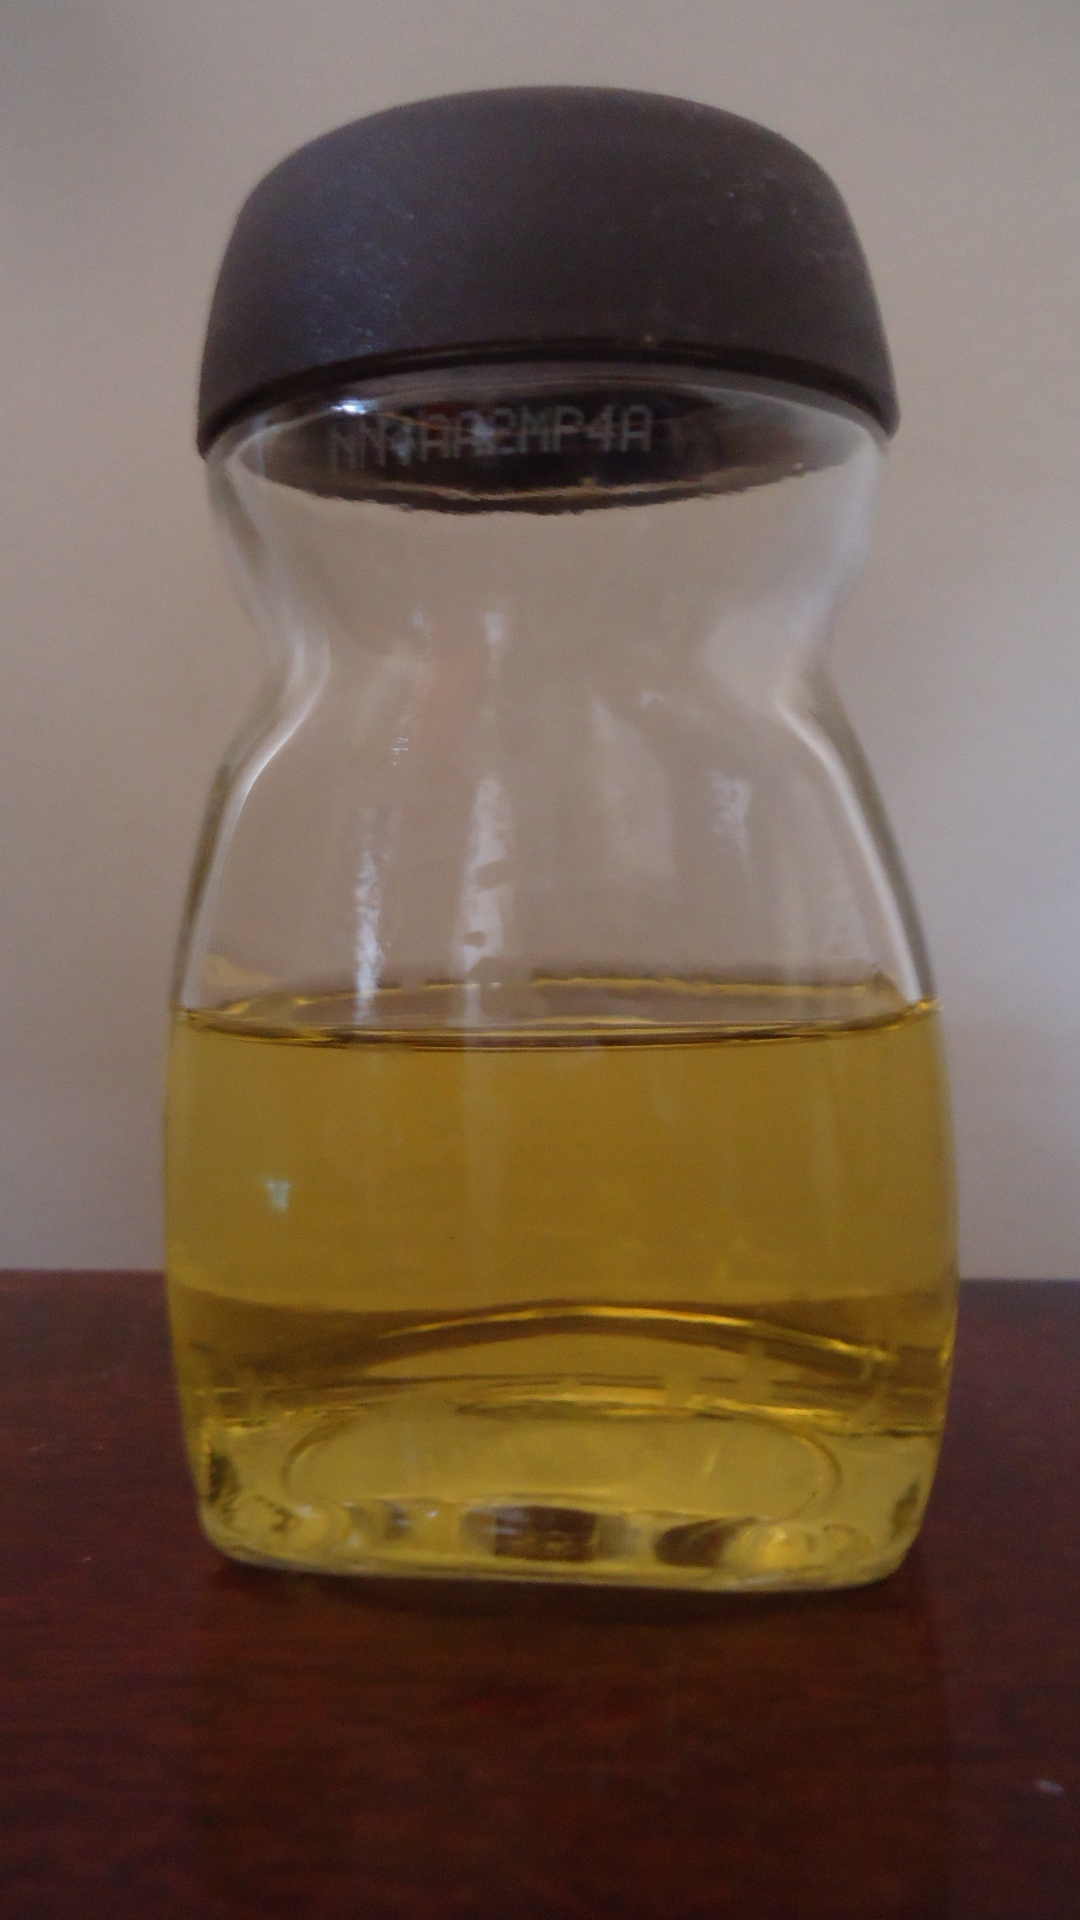
\includegraphics[scale=0.1]{imgs/oleo_essencial.jpg} 
	\end{minipage}
	\begin{minipage}{0.49\textwidth}
		\begin{itemize}
			\item Geraniol \pause
				\begin{itemize}
					\item Perfumaria \pause
					\item Ação antibacteriana (\emph{Salmonella typhimurium}) \cite{kim1995} \pause
					\item Repelente de insetos \cite{barnard2004} \pause
				\end{itemize}
			\item Citronelol \pause
				\begin{itemize}
					\item Perfumaria (Pode causar alergia em pessoas sensíveis) \pause
					\item Repelente de insetos \pause
				\end{itemize}
			\item Citronelal \pause
				\begin{itemize}
					\item Odor de limão \pause
					\item Repelente (Grande eficácia contra mosquitos) \cite{kim2005} \pause
					\item Antifúngico \cite{nakahara2003}
				\end{itemize}
		\end{itemize}
		
	\end{minipage}
\end{frame}

% ----------------- NOVO SLIDE --------------------------------
\section{Controle de carrapatos em bovinos}
\begin{frame}
\frametitle{Controle de carrapatos em bovinos}
	
	\begin{itemize}
		\item Perdas econômicas - 2 bilhões de dólares por ano \cite{grisi2002}
		
			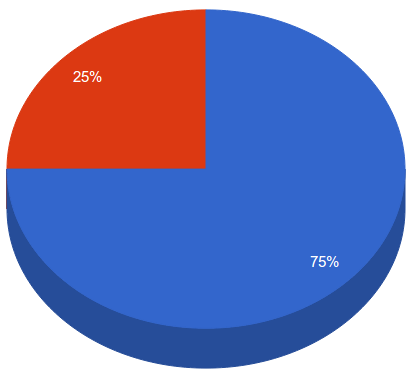
\includegraphics[scale=0.3]{imgs/grafico_perdas_economicas.png} 
			
			\color{blue}{75\% -- Carrapatos}
			
			\color{red}{25\% -- Outros parasitas}
	\end{itemize}
	
\end{frame}

% ----------------- NOVO SLIDE --------------------------------
\begin{frame}
\frametitle{Controle de carrapatos em bovinos}
	
	\begin{itemize}
		\item Produtos químicos causam danos ao bovino \cite{chagas2003}
		
		
		\item \citeauthor{clair2008} em \citeyear{clair2008}
		\begin{itemize}

			\item Óleo de citronela é acaricida \pause
			\item Eficácia contra o carrapato \pause
			\item Não tóxico \pause
			\item Concentrações baixas (6,1\% a 4.1\%).
					
		\end{itemize}
	\end{itemize}
	
\end{frame}

%

% ----------------- NOVO SLIDE --------------------------------
\section{Referências}

% --- O comando \allowframebreaks ---
% Se o conteúdo não se encaixa em um quadro, a opção allowframebreaks instrui 
% beamer para quebrá-lo automaticamente entre dois ou mais quadros,
% mantendo o frametitle do primeiro quadro (dado como argumento) e acrescentando 
% um número romano ou algo parecido na continuação.

\begin{frame}[allowframebreaks]{Referências}
\bibliography{referencias}
\end{frame}

% ----------------- FIM DO DOCUMENTO -----------------------------------------
\end{document}
